\documentclass{acmart}
\usepackage[utf8]{inputenc}
\usepackage{subfig}
\usepackage{graphicx}
\usepackage{sidebyside}
\usepackage{cleveref}
\usepackage{placeins}
\usepackage{colortbl}

\title{An inquiry into the influence of parallelism and the choice of random
engines on the runtime and results of Stride}

\author{Niels Aerens}
\author{Thomas Avé}
\author{Tobia De Koninck}
\author{Robin Jadoul}

% \date{March 2018}

\begin{abstract}
    In this article, we investigate a few properties of the Stride project. In particular, we look at the influence of the amount of parallelization with respect to the running time of a simulation and the difference in simulation outcomes when varying the used random number generator.
\end{abstract}

\begin{document}

\maketitle

\section{Introduction}
Stride \cite{KUYLEN20172438} is an individual-based Simulator for the Transmission of Infectious Diseases with focus on model flexibility and
performance. The performance of such a simulator is important for the researcher to have fast feedback in order to
build a reasonable model of the disease. The Stride program currently has scenario tests to prevent regressions in the
simulation output. To provide fast feedback to the developers working on Stride the test should run sufficiently quickly.
The running time of the tests are a good indication of the running time of the simulator itself. Hence we perform a
performance analysis of the running time of tests and the influence of parallelism.

The scenario tests are using the Attack Rate as parameter to assert the simulator outcome. Since Stride is a stochastic
system and thus relies on randomness, the output of its tests are variable. Therefore the tests use an acceptability range
for the test outcome. We determined these ranges by running the tested simulations multiple times (100+). We noticed
using a QQ-Plot and hypothesis tests that the Attack Rate can be considered to follow a normal distribution.
For the accepted ranges, we decided to allow a distance of 2 standard deviations from the observed mean.

The second topic of this paper is to analyze the influence of the random number generator engine on the Attack Rate.
Stride uses the Trng library \cite{bauke2015tina} as random number generator. The inspected engines are \texttt{lgc64}, \texttt{lgc64\_shift}, \texttt{mrg2}, \texttt{mrg3}, \texttt{yarn2} and \texttt{yarn3}.

\pagebreak

\section{Methods}

\subsection{Influence of multi-threading}

The analysis described in this section was performed on a 32 core AMD machine. Therefore the tests were executed with a maximum of 32 threads, which is a reasonable maximum for any workstation at time of writing. By using a Bash-script\footnote{\url{https://github.com/LEDfan/Bachelorproef/blob/597e9d14356a40f10c52dbd789ce495f0891720e/assets/src/week3/bench.sh}} % TODO update links to website
the Stride tests were run with an increasing amount of threads, starting at 1 up to 32.

\subsection{Influence of random engine}

Using a Python3 script\footnote{\url{https://github.com/LEDfan/Bachelorproef/blob/b8b67f7083ba8a523bdb16f0c6fd0fdfeea7dacf/assets/src/week3/random_engines.py}} % TODO update links to website
the simulation was run using the different random engines, at the same time the running time
was measured.

\section{Results}

\subsection{Influence of multi-threading}
The running time in function of the number of threads are shown in \cref{fig:threads}. The difference between the first and third
quartile is only 0.45 seconds. This difference is negligible compared to the 27 seconds running time. We can conclude
that the parallelisation of the code doesn’t have a great influence on the performance.
Note that for each number of threads, the values are obtained by running the Influenza A simulation 15 times and taking the average running time.

\sidebyside[!hbt][fig:threads:scatter][fig:threads:boxplot]
    {Connected scatter plot}
    {images/performance_scatter.png}
    {Boxplot}
    {images/boxplot_performance.png}
    {Running time in function of number of threads}
    {fig:threads}
\subsection{Influence of random engine}
The engine which needs the least amount of time is the \texttt{lgc64} engine, the \texttt{yarn3} engine needs the most time. The difference in time is 60 seconds when running the tests 15 times, which means that for one run the difference is only about 6 seconds. Thus there isn’t a big difference. A complete comparison of running times can be found in \cref{fig:engine:running}.


\begin{figure}
    \centering
    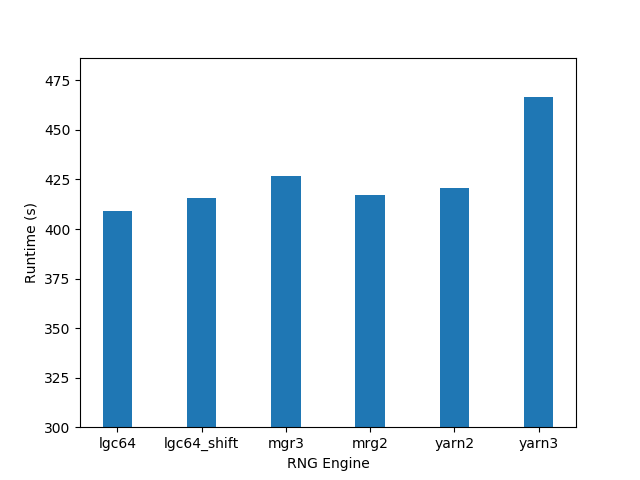
\includegraphics[width=0.7\textwidth]{images/engine_performance_bar.png}
    \caption{Running time of the different rng engines for the influenza A test case.}
    \label{fig:engine:running}
\end{figure}


The first test case of Stride (Influenza A\footnote{\url{https://github.com/LEDfan/Bachelorproef/blob/dd1ef48867238d62446813f47d6718908505b7f2/test/cpp/gtester/BatchRuns.cpp\#L82}})
performs a simulation of influenza in Flanders, with an $R_0$ value\footnote{Basic reproduction number, a measure for the infectiousness of a disease: the amount of people will 1 infected person infect directly in a completely
susceptible population.} of 3.0. For this test case the range of allowed attack rates doesn't change much. 
% TODO insert text about hypothesis tests
The second test case (Influenza B\footnote{\url{https://github.com/LEDfan/Bachelorproef/blob/dd1ef48867238d62446813f47d6718908505b7f2/test/cpp/gtester/BatchRuns.cpp\#L86}}) uses a seeding rate of 0, which results in a constant attack rate of 0. As expected the RNG engine doesn't have influence on this outcome.
The same holds for the third test case (Influenza C\footnote{\url{https://github.com/LEDfan/Bachelorproef/blob/dd1ef48867238d62446813f47d6718908505b7f2/test/cpp/gtester/BatchRuns.cpp\#L91}}) which uses very low seeding rate and a large immunity factor. The attack vector for every engine is 5.
The Measles 16\footnote{\url{https://github.com/LEDfan/Bachelorproef/blob/dd1ef48867238d62446813f47d6718908505b7f2/test/cpp/gtester/BatchRuns.cpp\#L97}} testcase is more interesting for the analysis of the RNG engines. The disease simulated is not influeanza but the measles. The $R_0$ value is set to 16, which results in a very large part of the population becoming infected.

% TODO insert text about hypothesis tests
The last testcase (Measles 60) sets the $R_0$ value to 60. It infects the whole population, so the attack rate is for all the engines the same.
    
\subsection{Normality of the output}
\label{par:normality}
To validate our assumption that the distribution of the attack rate was normal for our tests, we both looked at QQ-plots of the outputs of different runs against a reference normal distribution with $\mu = \bar{X}, \sigma=S_X$, verified that histograms had a more or less normal look to them, and verified with the Shapiro-Wilkes test.

% Influenza A
Looking at the Influenza A testcase, we find the resulting P-values for Shapiro-Wilkes test in \cref{tab:influenza_a:shapiro}. Here, all random engines result in an (at least approximately) normal distribution for the attack rate.
\begin{table}[!hbt]
    \begin{tabular}{c c c c c c}
       \textbf{lgc64} & \textbf{lgc64\_shift} & \textbf{mrg2} & \textbf{mrg3} & \textbf{yarn2} & \textbf{yarn3}\\
        0.2530 & 0.8561 & 0.2717 & 0.3722 & 0.4837 & 0.6319
    \end{tabular}
    \caption{P-values of the Influenza A test case for the Shapiro-Wilkes normality test}
    \label{tab:influenza_a:shapiro}
\end{table}


% Measles 16
For the Measles 16 testcase, resulting P-values for the Shapiro-Wilkes test can be found in \cref{tab:measles_16:shapiro}.
We can observe that only the \texttt{lgc64} engine fails the test at $p = 0.05$. % TODO: reference plots

\begin{table}[!hbt]
    \begin{tabular}{c c c c c c}
       \textbf{lgc64} & \textbf{lgc64\_shift} & \textbf{mrg2} & \textbf{mrg3} & \textbf{yarn2} & \textbf{yarn3}\\
        $1.039\times10^{-7}$ & 0.5460 & 0.1423 & 0.7592 & 0.2702 & 0.1516
    \end{tabular}
    \caption{P-values of the Measles 16 test case for the Shapiro-Wilkes normality test}
    \label{tab:measles_16:shapiro}
\end{table}

\subsection{Equality of acceptable ranges for the test cases}

In this section the equality of the different value ranges which are accepted by the tests for each random engine is verified. Only the Influenza A and Measles 16 test cases are studied since they provide have a variable range. The tests are done using t-test for the standard deviations and z-test for the means, since it's known that the data is normally distributed.

The hypotheses for the t-test:
\[
\begin{aligned}
 H_0 &: \sigma = \sigma_2\\
 H_1 &: \sigma \ne \sigma_2\
\end{aligned}
\]

and for the z-test:
\[
\begin{aligned}
 H_0 &: \mu_1 = \mu_2  \\
 H_1 &: \mu_1 \ne \mu_2.
\end{aligned}
\]

The p-values for these tests are listed in \cref{tab:measles_16:p_values} and clearly indicates that the \(H_0\) holds for both tests. % TOD update


\begin{table}[!hbt]
    \centering
    \bgroup
    \def\arraystretch{2}
    \begin{tabular}{c|c|c|c|c|c}
                                & \textbf{Influenza A}  & \textbf{Measles 16} \\ \hline
        \texttt{lgc64}          & \([1855,2279]\)       & \([588591,591128]\) \\
        \texttt{lgc64\_shift}   & \([1954,2226]\)       & \([588899,591513]\) \\
        \texttt{mrg2}           & \([1859,2415]\)       & \([589230,591369]\) \\
        \texttt{mrg3}           & \([1985,2329]\)       & \([589401,591198]\) \\
        \texttt{yarn2}          & \([1876,2331]\)       & \([588739,591488]\) \\
        \texttt{yarn3}          & \([1955,2300]\)       & \([589066,590965]\) \\
    \end{tabular}
    \egroup
    \caption{The acceptable attack rates for the Influenza A en Measles 16 test case for every random number engine}
    \label{tab:ranges_engines}
\end{table}

\begin{table}[!hbt]
    \begin{tabular}{c|c|c|c|c|c|c}
        & \textbf{lgc64\_shift} & \textbf{mrg2} & \textbf{mrg3} & \textbf{yarn2} \\
        \textbf{mrg2}      
            & \(p_{\mu} = 0.2337 \quad p_{\sigma} = 0.2217 \) 
            & \cellcolor{gray}
            & \cellcolor{gray}
            & \cellcolor{gray} \\
        \textbf{mrg3}          
            & \(p_{\mu} = 0.01715 \quad p_{\sigma} = 0.0234 \)
            & \(p_{\mu} = 0.6365 \quad p_{\sigma} = 0.703 \) 
            & \cellcolor{gray} 
            & \cellcolor{gray} \\
        \textbf{yarn2}        
            & \(p_{\mu} = 0.6767 \quad p_{\sigma} = 0.6782 \)  
            & \(p_{\mu} = 0.4729 \quad p_{\sigma} = 0.4849 \)  
            & \(p_{\mu} = 0.1485 \quad p_{\sigma} = 0.1613  \)  
            & \cellcolor{gray} \\
        \textbf{yarn3}          
            & \(p_{\mu} = 0.1798 \quad p_{\sigma} = 0.3083 \)  
            & \(p_{\mu} = 0.8226 \quad p_{\sigma} = 0.5178  \) 
            & \(p_{\mu} = 0.3502 \quad p_{\sigma} = 0.4936  \)
            & \(p_{\mu} = 0.5187 \quad p_{\sigma} = 0.5178  \) \\
    \end{tabular}
    \caption{P-values of the Influenza A test case}
    \label{tab:measles_16:p_values}
\end{table}


\begin{table}[!hbt]
    \begin{tabular}{c|c|c|c|c|c|c}
        & \textbf{lgc64\_shift} & \textbf{mrg2} & \textbf{mrg3} & \textbf{yarn2} \\
        \textbf{mrg2}      
            & \(p_{\mu} = 0.6677 \quad p_{\sigma} = 0.7113 \) 
            & \cellcolor{gray}
            & \cellcolor{gray}
            & \cellcolor{gray} \\
        \textbf{mrg3}          
            & \(p_{\mu} = 0.6488 \quad p_{\sigma} = 0.6813 \)
            & \(p_{\mu} = 0.9985 \quad p_{\sigma} = 0.9983 \) 
            & \cellcolor{gray} 
            & \cellcolor{gray} \\
        \textbf{yarn2}        
            & \(p_{\mu} = 0.7061 \quad p_{\sigma} = 0.7513 \)  
            & \(p_{\mu} = 0.4081 \quad p_{\sigma} = 0.3292 \)  
            & \(p_{\mu} = 0.3812  \quad p_{\sigma} = 0.3917  \)  
            & \cellcolor{gray} \\
        \textbf{yarn3}          
            & \(p_{\mu} = 0.3615 \quad p_{\sigma} = 0.3908  \)  
            & \(p_{\mu} = 0.124 \quad p_{\sigma} = 0.1112  \) 
            & \(p_{\mu} = 0.0929 \quad p_{\sigma} = 0.1258  \)
            & \(p_{\mu} = 0.6495 \quad p_{\sigma} = 0.65  \) \\
    \end{tabular}
    \caption{P-values of the Measles 16 test case}
    \label{tab:measles_16:p_values}
\end{table}

\clearpage

\begin{figure}%
   	\makebox[\textwidth][c]{%
   		\centering%
   		\subfloat[Boxplot of Influenza A run with \texttt{lgc64}]{%
   			{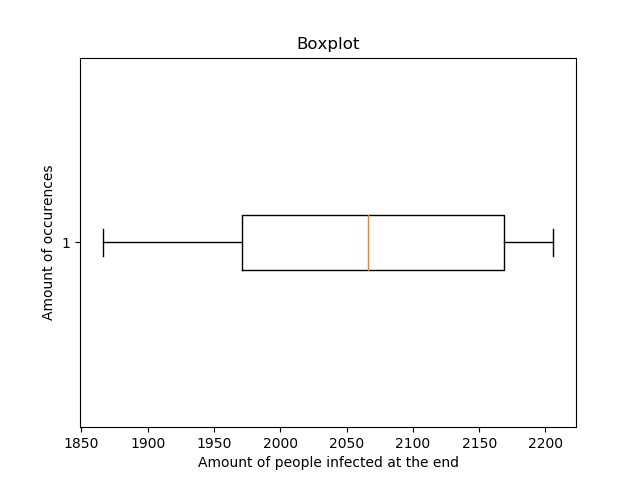
\includegraphics[width=0.5\textwidth]{images/boxplot_lgc64.png}}%
   		}%
   		\qquad%
   		\subfloat[Boxplot of Influenza A run with \texttt{lgc64\_shift}]{%
  			{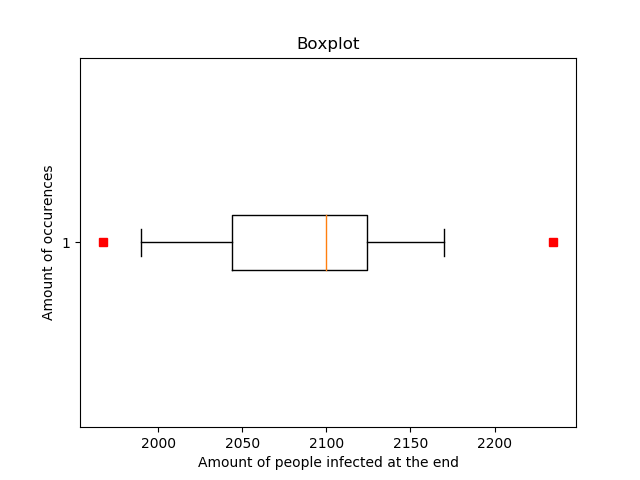
\includegraphics[width=0.5\textwidth]{images/boxplot_lgc64_shift.png}}%
   		}%
   	}\\
   	\makebox[\textwidth][c]{%
   		\centering%
   		\subfloat[Boxplot of Influenza A run with \texttt{mrg2}]{%
   			{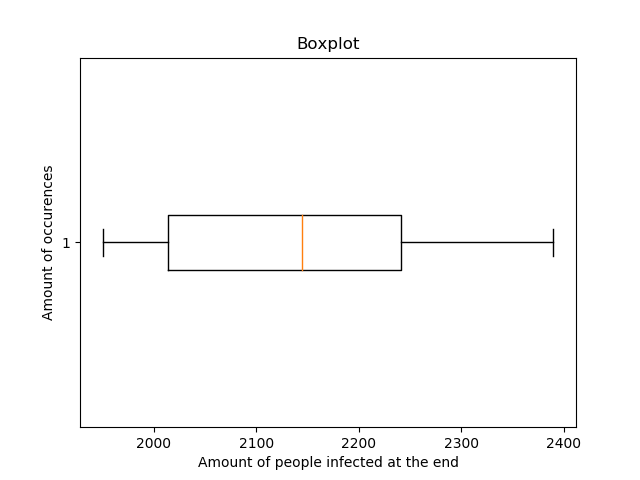
\includegraphics[width=0.5\textwidth]{images/boxplot_mrg2.png}}%
   		}%
   		\qquad%
   		\subfloat[Boxplot of Influenza A run with \texttt{mrg3}]{%
  			{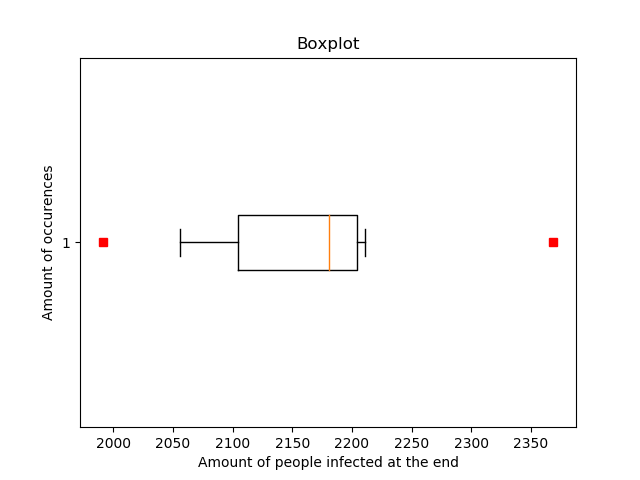
\includegraphics[width=0.5\textwidth]{images/boxplot_mrg3.png}}%
   		}%
   	}\\
   	\makebox[\textwidth][c]{%
   		\centering%
   		\subfloat[Boxplot of Influenza A run with \texttt{yarn2}]{%
   			{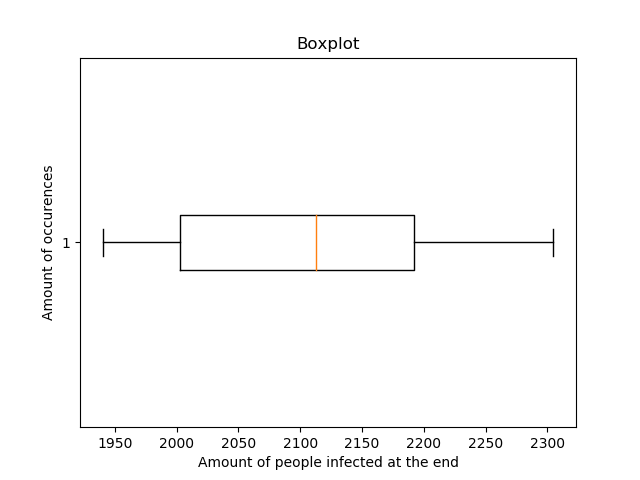
\includegraphics[width=0.5\textwidth]{images/boxplot_yarn2.png}}%
   		}%
   		\qquad%
   		\subfloat[Boxplot of Influenza A run with \texttt{yarn3}]{%
  			{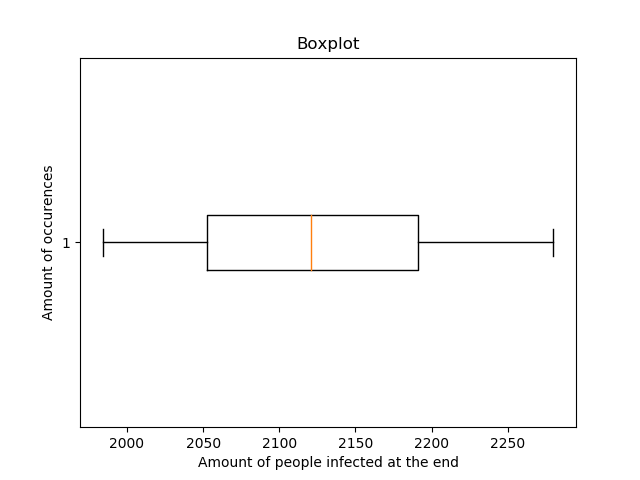
\includegraphics[width=0.5\textwidth]{images/boxplot_yarn3.png}}%
   		}%
   	}%
   	\caption{Running time in function of number of threads}
   	
\end{figure}

% TODO: investigate influence of threading on attack rate (hopefully minimal)

\clearpage

\bibliographystyle{ACM-Reference-Format}
\bibliography{references.bib}

\end{document}
